\subsection{高斯消元法与矩阵}

关于线性方程组的求解,有十分悠久的历史,我国古代名著《九章算术》就记载了求解线性方程组的一般方法,理论上的表述因德国数学家卡尔·高斯\footnote{卡尔·弗里德里希·高斯( 1777-1855)被许多人认为是有史以来最伟大的数学家之一,他令人惊叹的职业生涯需要数卷来记录。他被同行尊称为“数学之王”。在高斯去世后,其中一位同行写道:“他的思维深人了数字、空间和自然的最深奥秘;他测量了星星的轨迹,地球的形态和力量;他内化了未来一个世纪数学科学的演变。”历史证明了这一说法的正确性。}( Carl Gauss) 而被称为现在一般称这种方法为高斯消元法,以表彰他广泛使用并推广了这一方法。由于这种消元技术是基础性的,我们开始研究这一主题时,首先学习如何应用这种方法来计算线性方程的解。在掌握了计算方面的内容后,我们将转向围绕线性系统的更为理论性的方面。

问题是要在可能的情况下,计算含\( n \)个未知量的\( m \)个线性代数方程组的公共解。

\[\begin{aligned}&a_{11}x_1+a_{12}x_2+\cdots+a_{1n}x_n=b_1,\\&a_{21}x_1+a_{22}x_2+\cdots+a_{2n}x_n=b_2,\\&a_{m1}x_1+a_{m2}x_2+\cdots+a_{mn}x_n=b_m,\end{aligned}\]

其中\( x_i \)是未知量,\( a_{ij} \)和\( b_i \)是已知常数。\( a_{ij} \)被称为方程组的\textbf{系数},\( b_i\)的集合被称为方程组的\textbf{右侧项}。对于任何这样的方程组,解的集合恰好有三种可能性。

\begin{bluebox}{解集合的三种可能性}
	\begin{itemize}[leftmargin=*, labelsep=0.5em, itemsep=0.5em, topsep=0.5em]
		\item[■] \textbf{唯一解}:存在一组且仅有一组 $x_{i}$ 的值,同时满足所有方程
		\item[■] \textbf{无解}:不存在一组 $x_{i}$ 的值,同时满足所有方程—解集为空
		\item[■] \textbf{无限多解}:存在无穷多组不同的 $x_{i}$ 值,同时满足所有方程。很容易证明,如果一个系统有多个解,那么它就有无穷多个解。例如,一个系统不可能有确切的两个不同的解。
	\end{itemize}
\end{bluebox}

处理线性方程组的一部分工作是确定这三种可能性中哪一种成立。另一部分任务是,如果解唯一,则计算该解;如果有多个解,则描述所有解的集合。

高斯消元法是一种可用于实现所有这些目标的工具。高斯消元法是一种有条理的过程,通过依次消去未知量,将一个方程组系统地转化为另一个更简单但等价的方程组(如果两个方程组具有相同的解集,则称为\textbf{等价}的),最终得到一个易于求解的方程组。消元过程依赖于三种简单的运算,通过这些运算可以将一个方程组转化为另一个等价的方程组。为了描述这些运算,令\( E_k \)表示第\( k \)个方程。
\[E_k:a_{k1}x_1+a_{k2}x_2+\cdots+a_{kn}x_n=b_k\]

且将该方程组写为
\[\mathcal{S}=\begin{Bmatrix}E_{1}\\E_{2}\\\vdots\\E_{m}\end{Bmatrix}.\]

对于线性方程组\( \mathcal{S} \),以下三种\textbf{初等运算}中的每一种都会得到一个等价的方程组\( \mathcal{S}' \)。

\textbf{(1)} 交换第\( i \)个和第\( j \)个方程。即,若
\[\mathcal{S}=\begin{Bmatrix}E_{1}\\\vdots\\E_{i}\\\vdots\\E_{j}\\\vdots\\E_{m}\end{Bmatrix}, \mathrm{then} \mathcal{S}^{\prime}=\begin{Bmatrix}E_{1}\\\vdots\\E_{j}\\\vdots\\E_{i}\\\vdots\\E_{m}\end{Bmatrix}. (1.2.1)\]

\textbf{(2)} 用自身的一个非零倍数替换第\( i \)个方程。即,
\[\left.\mathcal{S}^{\prime}=\left\{\begin{array}{c}E_1\\\vdots\\\alpha E_i\\\vdots\\E_m\end{array}\right.\right\}, \mathrm{where} \alpha\neq0. (1.2.2)\]

\textbf{(3)} 用自身与第\( i \)个方程的一个倍数之和来替换第\( j \)个方程。即,
\[\left.S^{\prime}=\left\{\begin{array}{c}E_1\\\vdots\\E_i\\\vdots\\E_j+\alpha E_i\\\vdots\\E_m\end{array}\right.\right\}.(1.2.3)\]

为何这些运算都不会改变解集的解释留作练习。

实际中最常见的问题是具有\( n \)个方程和\( n \)个未知量的情况——称为\(\textbf{方形方程组}\),其有唯一解。由于高斯消元法在这种情况下较为直接,我们从这里开始,之后再讨论其他可能性。接下来详细描述将高斯消元法应用于以下简单(但典型)的方形方程组的过程:

\[\begin{aligned}2x+y+z=1,\\6x+2y+z=-1,\\-2x+2y+z=7.\end{aligned} (1.2.4)\]

在每一步中,策略是聚焦于一个称为\(\textbf{主元位置}\)的位置,并使用三种初等运算消去该位置下方的所有项。主元位置上的系数称为\(\textbf{主元元素}\)(或简称为\(\textbf{主元}\)),而主元所在的方程被称为\(\textbf{主元方程}\)。仅允许非零数作为主元。如果主元位置上的系数为0,则将主元方程与主元方程下方的某个方程交换,以得到非零主元。(对于具有唯一解的方形方程组,这总是可行的。)除非为0,否则第一个方程的第一个系数被选作第一个主元。例如,下方方程组中带圈的\textcircled{2}是第一步的主元:

\[\begin{array}{rcrcrcr}\textcircled{2}x&+&y&+&z&=&1,\\6x&+&2y&+&z&=&-1,\\-2x&+&2y&+&z&=&7.\end{array}\]

\textbf{步骤1.} 消去第一个主元下方的所有项。
\begin{itemize}
	\item 用第二个方程减去第一个方程的三倍,得到等价方程组:
\end{itemize}

\[
\begin{cases}
	\textcircled{2}x + y + z = 1, \\
	\quad - y - 2z = -4 \quad (E_2 - 3E_1), \\
	-2x + 2y + z = 7.
\end{cases}
\]

\begin{itemize}
	\item 将第一个方程加到第三个方程上,得到等价方程组:
\end{itemize}
\[
\begin{cases}
	\textcircled{2}x + y + z = 1, \\
	\quad - y - 2z = -4, \\
	\quad\quad 3y + 2z = 8 \quad (E_3 + E_1).
\end{cases}
\]

\textbf{步骤2.} 选择一个新的主元。
\begin{itemize}
	\item 暂时,通过向下并向右移动来选择一个新的主元\footnote{在数值计算中,选择主元的策略通常比单纯使用右下侧的下一个系数要复杂一些。目前先使用右下侧策略,之后会讨论更实用的策略。}。 若该系数不为0,则它是下一个主元。否则,与该位置下方的某个方程交换,以便将一个非零数带入该主元位置。在我们的例子中,$-1$是如下标识的第二个主元:
\end{itemize}
\[
\begin{cases}
	2x + y + z = 1, \\
	\textcircled{-1}y - 2z = -4, \\
	3y + 2z = 8.
\end{cases}
\]

\textbf{步骤3.} 消去第二个主元下方的所有项。
\begin{itemize}
	\item 将第二个方程的三倍加到第三个方程上,得到等价方程组:
\end{itemize}
\[
\begin{cases}
	2x + y + z = 1, \\
	\textcircled{-1}y - 2z = -4, \\
	-4z = -4 \quad (E_3 + 3E_2).
\end{cases}
\tag{1.2.5}
\]

\begin{itemize}
	\item 一般来说,在每一步中,你向下并向右移动以选择下一个主元,然后消去主元下方的所有项,直到无法继续进行。在本例中,第三个主元是\(-4\),但由于第三个主元下方没有需要消去的项,该过程完成。
\end{itemize}

此时,我们称该方程组已被\(\textbf{三角化}\)。三角方程组可通过一种称为\(\textbf{回代}\)的简单方法轻松求解,即先解最后一个方程得到最后一个未知量的值,然后将其代回倒数第二个方程,进而求解倒数第二个未知量,依此类推,直到每个未知量都被确定。对于我们的例子,解\((1.2.5)\)中的最后一个方程可得

\[ z = 1. \]

将\( z = 1 \)代回\((1.2.5)\)中的第二个方程并确定

\[ y = 4 - 2z = 4 - 2(1) = 2. \]

最后,将\( z = 1 \)和\( y = 2 \)代回\((1.2.5)\)中的第一个方程,得到

\[ x = \frac{1}{2}(1 - y - z) = \frac{1}{2}(1 - 2 - 1) = -1, \]

这就完成了求解。

显然,在每一步中,我们没有必要写下诸如“\( x \)”“\( y \)”“\( z \)”和“\( = \)”之类的符号,因为我们仅在处理系数。如果舍弃这些符号,线性方程组就简化为一个矩形数阵,其中每一行代表一个方程。例如,\((1.2.4)\)中的方程组可简化为如下数阵:

\[\begin{pmatrix}2&1&1&&1\\6&2&1&&-1\\-2&2&1&&7\end{pmatrix}. \text{(这条竖线强调了原来等号出现的位置。)}\]

系数的数阵——竖线左侧的数——被称为该方程组的\(\boxed{\text{系数矩阵}}\)。整个数阵——由方程组右侧的数扩充得到的系数矩阵——被称为与该方程组相关的\(\boxed{\text{增广矩阵}}\)。若系数矩阵记为\(\mathbf{A}\),右侧(常数列)记为\(\mathbf{b}\),则与该方程组相关的增广矩阵记为\([\mathbf{A}|\mathbf{b}]\)。

形式上,\textbf{标量}(scalar)是实数或复数,\textbf{矩阵}(matrix)是标量的矩形数阵。通常的惯例是用\textbf{大写粗体字母}表示矩阵,用对应的\textbf{带两个下标的小写字母}表示矩阵中的单个元素。例如,

\[
\mathbf{A} = \begin{pmatrix}
	a_{11} & a_{12} & \cdots & a_{1n} \\
	a_{21} & a_{22} & \cdots & a_{2n} \\
	\vdots & \vdots & \ddots & \vdots \\
	a_{m1} & a_{m2} & \cdots & a_{mn}
\end{pmatrix}.
\]

矩阵中单个元素的第一个下标指明该元素所在的\(\boxed{\text{行}}\)(水平线),第二个下标指明该元素所在的\(\boxed{\text{列}}\)(垂直线)。例如,若

\[\mathbf{A}=\begin{pmatrix}2&1&3&4\\8&6&5&-9\\-3&8&3&7\end{pmatrix}, \mathrm{then} a_{11}=2,a_{12}=1,\ldots,a_{34}=7. (1.2.6)\]

给定矩阵\(\mathbf{A}\)的\(\boxed{\text{子矩阵}}\)(submatrix)是通过删除\(\mathbf{A}\)的任意行和列组合得到的数阵。例如,\(\mathbf{B} = \begin{pmatrix} 2 & 4 \\ -3 & 7 \end{pmatrix}\)是\((1.2.6)\)中矩阵\(\mathbf{A}\)的子矩阵,因为\(\mathbf{B}\)是删除\(\mathbf{A}\)的第二行以及第二、三列后得到的结果。

当矩阵\(\mathbf{A}\)恰好有\( m \)行和\( n \)列时,称其\(\boxed{\text{形状}}\)或\(\boxed{\text{规模}}\)为\( m \times n \)(读作“\( m \) 乘 \( n \)”)。例如,\((1.2.6)\)中的矩阵是一个\( 3 \times 4 \)矩阵。按照约定,\( 1 \times 1 \)矩阵与标量视为同一对象,反之亦然。为了强调矩阵\(\mathbf{A}\)的形状是\( m \times n \),有时会给\(\mathbf{A}\)添加下标记为\(\mathbf{A}_{m \times n}\)。当\( m = n \)时(即\(\mathbf{A}\)的行数与列数相同),\(\mathbf{A}\)称为\(\boxed{\text{方阵}}\);否则,\(\mathbf{A}\)称为\(\boxed{\text{矩形矩阵}}\)。仅由一行或一列组成的矩阵通常分别称为\(\boxed{\text{行向量}}\)或\(\boxed{\text{列向量}}\)。

符号\(\mathbf{A}_{i*}\)用于表示第\( i \)行,而\(\mathbf{A}_{*j}\)表示矩阵\(\mathbf{A}\)的第\( j \)列。例如,若\(\mathbf{A}\)是\((1.2.6)\)中的矩阵,则

\[\mathbf{A}_{2*}=\begin{pmatrix}8&6&5&-9\end{pmatrix} \mathrm{and} \mathbf{A}_{*2}=\begin{pmatrix}1\\6\\8\end{pmatrix}.\]

对于一个线性方程组

\[\begin{aligned}&a_{11}x_1+a_{12}x_2+\cdots+a_{1n}x_n=b_1,\\&a_{21}x_1+a_{22}x_2+\cdots+a_{2n}x_n=b_2,\\&a_{m1}x_1+a_{m2}x_2+\cdots+a_{mn}x_n=b_m,\end{aligned}\]

高斯消元法可通过对相关增广矩阵\([\mathbf{A}|\mathbf{b}]\)的行执行**初等行变换**来实施,这些行变换对应于处理线性方程组时所用的三种初等运算\((1.2.1)\)、\((1.2.2)\)和\((1.2.3)\)。对于一个\( m \times n \)矩阵

\[\mathbf{M}=\begin{pmatrix}\mathbf{M}_{1*}\\\vdots\\\mathbf{M}_{i*}\\\vdots\\\mathbf{M}_{j*}\\\vdots\\\mathbf{M}_{m*}\end{pmatrix},\]

对矩阵\(\mathbf{M}\)的三种\(\boxed{\text{初等行变换}}\)(elementary row operations)类型如下。

- 类型I:交换第\( i \)行和第\( j \)行,得到
\[
\begin{pmatrix}
	\mathbf{M}_{1*} \\
	\vdots \\
	\mathbf{M}_{j*} \\
	\vdots \\
	\mathbf{M}_{i*} \\
	\vdots \\
	\mathbf{M}_{m*}
\end{pmatrix}
\tag{1.2.7}
\]

- 类型II:用自身的一个非零倍数替换第\( i \)行,得到
\[
\begin{pmatrix}
	\mathbf{M}_{1*} \\
	\vdots \\
	\alpha\mathbf{M}_{i*} \\
	\vdots \\
	\mathbf{M}_{m*}
\end{pmatrix}, \quad \text{where} \quad \alpha \neq 0.
\tag{1.2.8}
\]

- 类型III:用自身加上第\( i \)行的一个倍数的组合替换第\( j \)行,得到
\[
\begin{pmatrix}
	\mathbf{M}_{1*} \\
	\vdots \\
	\mathbf{M}_{i*} \\
	\vdots \\
	\mathbf{M}_{j*} + \alpha\mathbf{M}_{i*} \\
	\vdots \\
	\mathbf{M}_{m*}
\end{pmatrix}.
\tag{1.2.9}
\]

用初等行变换求解方程组(1.2.4)时,从相关的增广矩阵\( [\mathbf{A}|\mathbf{b}] \)开始,通过执行与对等式本身执行的初等运算完全对应的同一系列行变换,将系数矩阵\( \mathbf{A} \)三角化:
\[
\left(
\begin{array}{ccc|c}
	\boxed{2} & 1 & 1 & 1 \\
	6 & 2 & 1 & -1 \\
	-2 & 2 & 1 & 7 \\
\end{array}
\right)
\xrightarrow[R_3 + R_1]{R_2 - 3R_1}
\left(
\begin{array}{ccc|c}
	2 & 1 & 1 & 1 \\
	0 & \boxed{-1} & -2 & -4 \\
	0 & 3 & 2 & 8 \\
\end{array}
\right)
\xrightarrow{R_3 + 3R_2}
\left(
\begin{array}{ccc|c}
	2 & 1 & 1 & 1 \\
	0 & -1 & -2 & -4 \\
	0 & 0 & -4 & -4 \\
\end{array}
\right)
\]

最终的数阵表示三角方程组
\[\begin{aligned}2x+y+z=1,\\-y-2z=-4,\\-4z=-4\end{aligned}\]

它可以通过前面描述的回代法求解。一般来说,如果一个\( n \times n \)的方程组已被三角化为如下形式
\[
\begin{pmatrix}
	t_{11} & t_{12} & \cdots & t_{1n} & \big| & c_1 \\
	0 & t_{22} & \cdots & t_{2n} & \big| & c_2 \\
	\vdots & \vdots & \ddots & \vdots & \big| & \vdots \\
	0 & 0 & \cdots & t_{nn} & \big| & c_n \\
\end{pmatrix}
\tag{1.2.10}
\]

其中每个\( t_{ii} \neq 0 \)(即没有零主元),那么回代的一般算法如下。
\begin{bluebox}{回代算法}
	从(1.2.10)中确定\( x_i \)的值,首先令\( x_n = c_n / t_{nn} \),然后递归计算
	\[
	x_i = \frac{1}{t_{ii}} \left( c_i - t_{i,i+1}x_{i+1} - t_{i,i+2}x_{i+2} - \cdots - t_{in}x_n \right)
	\]
	其中\( i = n-1, n-2, \ldots, 2, 1 \)。
\end{bluebox}

评估算法效率的一种方法是统计所需的算术运算次数\footnote{仅靠运算次数来评估算法的效率,可能不再像过去那样重要了。老式计算机按顺序执行指令,而一些现代机器能够并行执行指令,因此不同的数值任务可以同时进行。适合并行化的算法可能运算次数更高,但在并行机器上的运行速度可能比运算次数较少但无法利用并行性的算法更快。仅靠运算次数来评估算法的效率,可能不再像过去那样重要了。老式计算机按顺序执行指令,而一些现代机器能够并行执行指令,因此不同的数值任务可以同时进行。适合并行化的算法可能运算次数更高,但在并行机器上的运行速度可能比运算次数较少但无法利用并行性的算法更快。}由于多种原因,加法和减法不做区分,乘法和除法也不做区分。此外,乘/除法通常与加/减法分开统计。即使你不深究细节,了解高斯消元法结合回代的运算次数也很重要,这样当遇到其他算法时,你就有了比较的依据。

\begin{bluebox}{高斯消元运算次数}
	对\( n \times n \)系统应用高斯消元结合回代,需要
	\[
	\frac{n^3}{3} + n^2 - \frac{n}{3} \quad \text{次乘/除法}
	\]
	和
	\[
	\frac{n^3}{3} + \frac{n^2}{2} - \frac{5n}{6} \quad \text{次加/减法}.
	\]
	当\( n \)增大时,\( n^3/3 \)项在这些表达式中占主导地位。因此,需要记住的重要点是,对\( n \times n \)系统进行高斯消元结合回代,大约需要\( n^3/3 \)次乘/除法,且加/减法的次数大致相同。
\end{bluebox}

% 红色文字
\textcolor{red}{例子1.2.1}
% 红色水平线(宽度为文本宽度,厚度0.4pt)
\color{red}\rule{\textwidth}{0.4pt}\color{black}

问题:用高斯消元结合回代法解下列方程组:
\[
\begin{cases}
	v - w = 3, \\
	-2u + 4v - w = 1, \\
	-2u + 5v - 4w = -2.
\end{cases}
\]

解:对应的增广矩阵为
\[
\begin{pmatrix}
	0 & 1 & -1 & \big| & 3 \\
	-2 & 4 & -1 & \big| & 1 \\
	-2 & 5 & -4 & \big| & -2
\end{pmatrix}.
\]

由于第一个主元位置是0,在消去第一个主元下方的元素之前,交换第一行和第二行:
\[
\begin{pmatrix}
	\boxed{0} & 1 & -1 & \big| & 3 \\
	-2 & 4 & -1 & \big| & 1 \\
	-2 & 5 & -4 & \big| & -2
\end{pmatrix}
\xrightarrow{\text{交换} R_1 \text{和} R_2}
\begin{pmatrix}
	\boxed{-2} & 4 & -1 & \big| & 1 \\
	0 & 1 & -1 & \big| & 3 \\
	-2 & 5 & -4 & \big| & -2
\end{pmatrix}
\xrightarrow{R_3 - R_1}
\begin{pmatrix}
	-2 & 4 & -1 & \big| & 1 \\
	0 & \boxed{1} & -1 & \big| & 3 \\
	0 & 1 & -3 & \big| & -3
\end{pmatrix}
\xrightarrow{R_3 - R_2}
\begin{pmatrix}
	-2 & 4 & -1 & \big| & 1 \\
	0 & 1 & -1 & \big| & 3 \\
	0 & 0 & -2 & \big| & -6
\end{pmatrix}
\]

回代得:

\[\begin{aligned}&w=\frac{-6}{-2}=3,\\&v=3+w=3+3=6,\\&u=\frac{1}{-2}\left(1-4v+w\right)=\frac{1}{-2}\left(1-24+3\right)=10.\end{aligned}\]

% 红色文字
\textcolor{red}{练习1.2}
% 红色水平线(宽度为文本宽度,厚度0.4pt)
\color{red}\rule{\textwidth}{0.4pt}\color{black}

\subsubsection{用高斯消元结合回代法解下列方程组:}
\[
\begin{cases}
	x_1 + x_2 + x_3 = 1, \\
	x_1 + 2x_2 + 2x_3 = 1, \\
	x_1 + 2x_2 + 3x_3 = 1.
\end{cases}
\]

\subsubsection{用高斯消元结合回代法解下列方程组:}
\[
\begin{cases}
	2x_1 - x_2 = 0, \\
	-x_1 + 2x_2 - x_3 = 0, \\
	-x_2 + x_3 = 1.
\end{cases}
\]
\subsubsection{用高斯消元结合回代法解下列方程组:}
\[
\begin{cases}
	4x_2 - 3x_3 = 3, \\
	-x_1 + 7x_2 - 5x_3 = 4, \\
	-x_1 + 8x_2 - 6x_3 = 5.
\end{cases}
\]

\subsubsection{解下列方程组:}
\[
\begin{cases}
	x_1 + x_2 + x_3 + x_4 = 1, \\
	x_1 + x_2 + 3x_3 + 3x_4 = 3, \\
	x_1 + x_2 + 2x_3 + 3x_4 = 3, \\
	x_1 + 3x_2 + 3x_3 + 3x_4 = 4.
\end{cases}
\]

\subsubsection{考虑以下三个系统,每个系统的系数相同,但右手边不同(这种情况经常出现):}
\[
\begin{cases}
	4x - 8y + 5z = 1 \big| 0 \big| 0, \\
	4x - 7y + 4z = 0 \big| 1 \big| 0, \\
	3x - 4y + 2z = 0 \big| 0 \big| 1.
\end{cases}
\]
通过对形式为\( [\mathbf{A} \mid \mathbf{b_1} \mid \mathbf{b_2} \mid \mathbf{b_3}] \)的增广矩阵执行高斯消元,一次性解出所有三个系统。

\subsubsection{假设矩阵\(\mathbf{B}\)是通过对矩阵\(\mathbf{A}\)执行一系列行变换得到的。解释为什么可以通过对\(\mathbf{B}\)执行行变换得到\(\mathbf{A}\)。}

\subsubsection{求满足以下条件的角\(\alpha\)、\(\beta\)和\(\gamma\):}
\[
\begin{cases}
	2\sin\alpha - \cos\beta + 3\tan\gamma = 3, \\
	4\sin\alpha + 2\cos\beta - 2\tan\gamma = 2, \\
	6\sin\alpha - 3\cos\beta + \tan\gamma = 9,
\end{cases}
\]
其中\(0 \leq \alpha \leq 2\pi\),\(0 \leq \beta \leq 2\pi\),且\(0 \leq \gamma < \pi\)。

\subsubsection{以下方程组无解:}
\[
\begin{cases}
	-x_1 + 3x_2 - 2x_3 = 1, \\
	-x_1 + 4x_2 - 3x_3 = 0, \\
	-x_1 + 5x_2 - 4x_3 = 0.
\end{cases}
\]
尝试用高斯消元法解这个方程组,并解释出现了什么情况表明该方程组无法求解。

\subsubsection{尝试用高斯消元法解方程组}
\[
\begin{cases}
	-x_1 + 3x_2 - 2x_3 = 4, \\
	-x_1 + 4x_2 - 3x_3 = 5, \\
	-x_1 + 5x_2 - 4x_3 = 6,
\end{cases}
\]
并解释为什么这个方程组一定有无穷多解。

\subsubsection{通过解一个\(3 \times 3\)方程组,求过点\((1,1)\)、\((2,2)\)和\((3,0)\)的抛物线\(y = \alpha + \beta x + \gamma x^2\)方程中的系数。}

\subsubsection{假设100只昆虫分布在一个由四个腔室组成的封闭空间中,腔室之间有如下所示的通道。}

\begin{figure}[h]
	\centering
	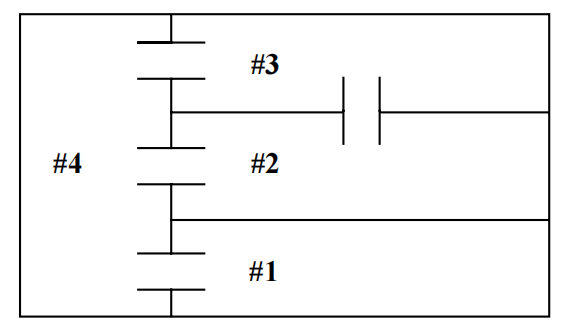
\includegraphics[width=\linewidth]{fig1.2.11} 
\end{figure}

一分钟后,昆虫重新分布。假设一分钟的时间不足以让一只昆虫访问超过一个腔室,且在一分钟结束时,每个腔室中40\%的昆虫没有离开它们在分钟开始时所处的腔室。离开一个腔室的昆虫会均匀分散到从其初始腔室可直接到达的腔室中——例如,从\#3出发,一半移向\#2,一半移向\#4。

(a) 若一分钟后,腔室\#1、\#2、\#3和\#4中分别有12、25、26和37只昆虫,确定初始分布必须是什么。

(b) 若初始分布是20、20、20、40,一分钟后的分布是什么?

\subsubsection{证明第8页讨论的三种初等行变换不独立,即通过(1.2.8)和(1.2.9)中的另外两种行变换序列可以完成交换操作(1.2.7)。}

\subsubsection{假设\([\mathbf{A}|\mathbf{b}]\)是线性系统的增广矩阵。你知道对\([\mathbf{A}|\mathbf{b}]\)执行行变换不会改变系统的解。然而,从未提及列操作,因为列操作会改变解。}
\begin{itemize}
	\item[(a)] 当列\(\mathbf{A}_{*j}\)和\(\mathbf{A}_{*k}\)交换时,描述对线性系统解的影响。
	\item[(b)] 当列\(\mathbf{A}_{*j}\)被\(\alpha\mathbf{A}_{*j}\)(\(\alpha \neq 0\))替换时,描述其影响。
	\item[(c)] 当列\(\mathbf{A}_{*j}\)被\(\mathbf{A}_{*j} + \alpha\mathbf{A}_{*k}\)替换时,描述其影响。
	提示:用2×2或3×3系统进行实验。
\end{itemize}

\subsubsection{考虑由下式定义的\(n \times n\)希尔伯特矩阵\(\mathbf{H}\):}
\[
\mathbf{H} = \begin{pmatrix}
	1 & \frac{1}{2} & \frac{1}{3} & \cdots & \frac{1}{n} \\
	\frac{1}{2} & \frac{1}{3} & \frac{1}{4} & \cdots & \frac{1}{n+1} \\
	\frac{1}{3} & \frac{1}{4} & \frac{1}{5} & \cdots & \frac{1}{n+2} \\
	\vdots & \vdots & \vdots & \cdots & \vdots \\
	\frac{1}{n} & \frac{1}{n+1} & \frac{1}{n+2} & \cdots & \frac{1}{2n-1}
\end{pmatrix}
\]
用\(i\)和\(j\)表示单个元素\(h_{ij}\)。

\subsubsection{验证文中给出的高斯消元结合回代法的运算次数对一般3×3系统是正确的。如果有挑战欲,尝试对一般\(n \times n\)系统验证这些次数。}

\subsubsection{解释为什么线性系统不可能恰好有两个不同的解。将你的论证扩展到解释:如果一个系统有多个解,那么它必须有无穷多个不同的解。}






















